\section{Authentication process}



\subsection{Process}

{\bf Network login phase}:
The first thing the client does is ask what protocol is supported. In this case the target responded and said please do NLA~\ref{windows:nla} The client then immediately prompts for credentials. Doesn't do anything special, just prompts.

Once the user enters their creds NLA kicks in. NLA is the first stage of the CredSSP~\ref{windows:credssp} protocol, which is how those creds you typed in make it to the target server securely. 

NLA works by first opening an SPNEGO~\ref{windows:spnego} Negotiate connection with the target.

The target happily responds and depending on a few conditions might do a couple different things:
\begin{itemize}
    \item first case [\href{https://www.thehacker.recipes/ad/movement/kerberos#user-to-user-authentication}{U2U}]: the target provides its machine account's Kerberos TGT. The client does a TGS-REQ asking for a TGS  to the target name \verb+termsrv/target.domain.com+, and passes the TGT into the \verb+additional-tickets+ field to do something called user-to-user or encrypt-in-session-key authentication
    \item second case [kerberos]: Si le client a utilisé le FQDN de la target, the client just requests a ticket to \verb+termsrv/target.domain.com+ the usual way
    \item third case [NTLMSSP]: Si le client a utilisé l'IP de la target, NTLM happens when
    \item fourth case [PKU2U~\ref{windows:pku2u}]: This is special to AAD-joined target machines only
\end{itemize}

The client converts the ticket to the target into an AP-REQ and fires it off to the target. The target receives it and decrypts it using either the session key in it's machine TGT, or using it's machine password

{\bf credential transfert phase}:
The target then generates a {\bf session key} and stashes it in a place LSA can get to. An AP-REP is returned to the client containing this session key

now CredSSP takes those creds and encrypts them using the session key. The client then fires this blob off to the target server.

And the target receives the blob. It takes the session key it stashed away a while back and decrypts the blob. Now it has a username and password. 

{\bf Interactive login phase}:
That username and password is passed to the logon UI bits and now we're back to that original thread.

There are some notable differences here though. For instance remote connections never go through cached logon.

\subsection{Smartcard and Windows Hello}

Smart Card-based CredSSP works similarly to passwords. The NLA portion works just the same. The difference is the creds themselves. It turns out RDP emulates the smart card hardware and literally passes hardware commands back and forth over the channel.

\subsection{Remote credential guard}
See~\ref{windows:remote_credential_guard}

\href{https://learn.microsoft.com/en-us/windows/security/identity-protection/remote-credential-guard?tabs=intune}{Remote Credential Guard (microsoft)}

\begin{figure}[!ht]
    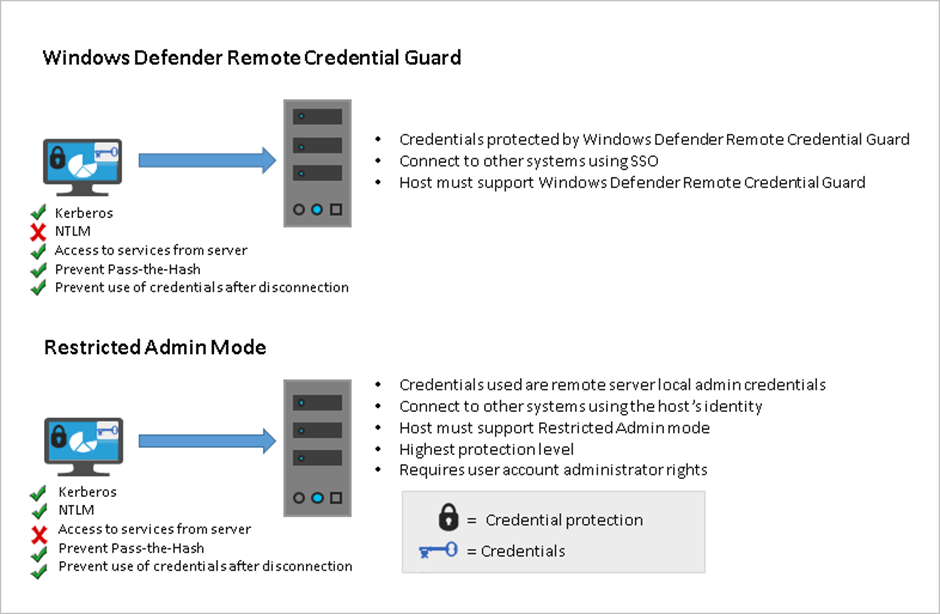
\includegraphics[width=\linewidth]{network/rdp/images/restrictedadmin-rcg.png}
    \caption{restrictedadmin-rcg}
    \label{fig:restrictedadmin-rcg}
\end{figure}

RCG works by creating a reverse proxy of sorts from the target to the client. Whenever an application on the target needs a ticket of some sort to something it asks LSA. LSA is aware of RCG and so it opens a channel back to the client.

Over the channel the target LSA asks the client to ask (ish) the client LSA for a ticket to whatever the target needs. The client obliges, and forwards the ticket. The target now has a ticket, and never saw the creds.

\subsection{PKU2U}

\subsection{Network Level Authent:ication (NLA)}
\label{windows:nla}

Network Level Authentication (NLA) is a feature of Remote Desktop Services (RDP Server) or Remote Desktop Connection (RDP Client) that requires the connecting user to authenticate themselves before a session is established with the server.

Originally, if a user opened an RDP (remote desktop) session to a server it would load the login screen from the server for the user. This would use up resources on the server, and was a potential area for denial of service attacks as well as remote code execution attacks (see BlueKeep). Network Level Authentication delegates the user's credentials from the client through a client-side Security Support Provider and prompts the user to authenticate before establishing a session on the server.


\subsection{Restricted admin}
See~\ref{windows:retricted_admin}

\href{https://learn.microsoft.com/en-us/previous-versions/windows/it-pro/windows-server-2012-r2-and-2012/dn283323(v=ws.11)}{What’s new in Remote Desktop Services in Windows Server 2012 R2}

Restricted Admin mode provides a method of interactively logging on to a remote host server without transmitting your credentials to the server. 

{\bf Note}: 
\begin{itemize}
    \item Once connected to a host in RestrictedAdmin mode, the user will not be able to seamlessly access other network resources from that host using the credentials they provided to the remote desktop client.
    \item Restricted Admin mode requires that the user be a member o the Local Administrators group on the RDP server.
\end{itemize}

Using this mode with administrator credentials, the remote desktop client attempts to interactively logon to a host that also supports this mode without sending credentials. When the host verifies that the user account connecting to it has administrator rights and supports Restricted Admin mode, the connection succeeds. Otherwise, the connection attempt fails. Restricted Admin mode does not at any point send plain text or other re-usable forms of credentials to remote computers.

vec l’utilisation du « Restricted Admin mode » ou « Mode d’administration Restreint » aucune informations d’identification ne sera stocké sur la machine distante qui peut potentiellement être compromise. De plus, il sera impossible de se connecter sur une autre machine de notre environnement sans saisir de nouveau le couple (identifiant + mot de passe). 


\subsection{Protected user and RDP}

Protected Users ajoute des protections sur la gestion de l’authentification :
\begin{itemize}
    \item Empeche de se loguer via NTLM
    \item Empeche le cache d'authentifiants
    \item Empeche l'utilisation de RC4 (NTLM) pour la    pré-authentification Kerberos 
\end{itemize}

NTLMSSP sera choisi si :
\begin{itemize}
    \item Le client n'appartient pas à un domaine OU
    \item Le client utilise l'adresse IP pour se connecter au serveur
\end{itemize}

Kerberos sera choisi si :
\begin{itemize}
    \item Le client et le serveur appartiennent au même domaine ET
    \item Le client utilise le FQDN du serveur pour la connexion
\end{itemize}

\subsection{links}

\begin{itemize}
    \item \href{https://syfuhs.net/how-authentication-works-when-you-use-remote-desktop}{How authentication works when you use remote desktop}
    \item \href{https://techcommunity.microsoft.com/t5/security-compliance-and-identity/azure-advanced-threat-protection-credssp-exploit-analysis/ba-p/250556}{Azure Advanced Threat Protection: CredSSP Exploit}
    \item \href{https://learn.microsoft.com/en-us/previous-versions/windows/it-pro/windows-10/security/threat-protection/security-policy-settings/network-security-allow-pku2u-authentication-requests-to-this-computer-to-use-online-identities}{Network security: Allow PKU2U authentication requests to this computer to use online identities}
    \item \href{https://awakecoding.com/posts/rdp-nla-with-azure-ad-the-pku2u-nightmare/}{RDP NLA with Azure AD: The PKU2U Nightmare}
    \item \href{https://cyber.gouv.fr/sites/default/files/IMG/pdf/Securite_de_RDP_article.pdf}{Sécurité de RDP}
    \item \href{https://www.sstic.org/media/SSTIC2020/SSTIC-actes/analyse_de_la_scurit_rdp__nla_quel_apport_pour_vot/SSTIC2020-Slides-analyse_de_la_scurit_rdp__nla_quel_apport_pour_votre_scurit_-bertoli_bourguenolle.pdf}{Sécurité RDP : Intecteption
    d’authentification sur NLA avec
    CredSSPy}
\end{itemize}